\subsection{Initialization of application}
%---------------------------
%include sequence diagram for initialization here
%---------------------------

\subsection{example action: select export format}
This sequence diagram states as example for a simple action handler.
In this action the user wants the currently displayed output translated into a specified format. The sequence diagram starts when the user selects the export format in the UI. 
The SelectExportFormat poses as action handler for the selected UI element. Thus when this element is clicked, the actions run() method is called. All invoked instances are already existing, none is being created in this scenario.
The actions run() method generates the dedicated representation by requesting the currently displayed lambda terms from the ExecutionEngine instance and generating their representation.
The representation is then written into the export window that will be displayed to the user. Writing before showing this export window ensures, that at no point in time an empty window is displayed.
However, before actually displaying it, a blocker that prevents the user from interacting with any UI element, other than the export window, is enabled.

\begin{figure}[H]
	\centering
	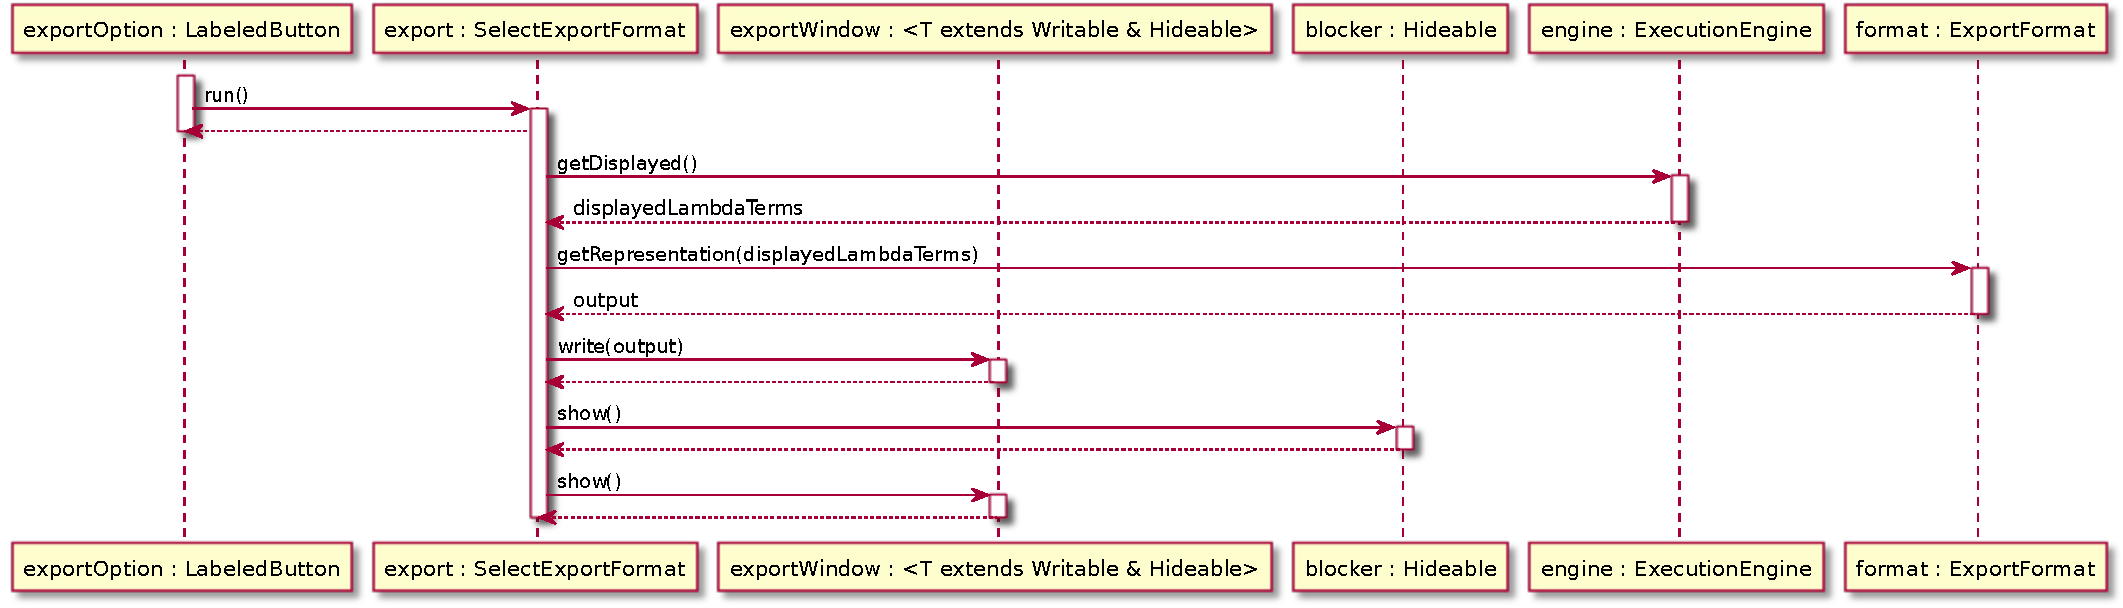
\includegraphics[width=\textwidth]{sequenceDiagrams/exportOutput}
	\caption{Sequence diagram for the select export format action.}
\end{figure}

\subsection{example action: select exercise from main menu}
The \texttt{\hyperref[type:edu.kit.wavelength.client.view.action.SelectExercise]{SelectExercise}} 
action handles the UI elements, when the user selects an exercise from the main menu.

This action only prepares the UI to display the content of the selected exercise, 
it does not load the actual content into the UI. If the content of the editor would 
be overridden when the selected exerciser is loaded, the action displays a warning
message. Otherwise it just calls the \texttt{\hyperref[type:edu.kit.wavelength.client.view.action.LoadExercise]{LoadExercise}} 
action which will in return load the selected exercise.

\begin{figure}[H]
	\centering
	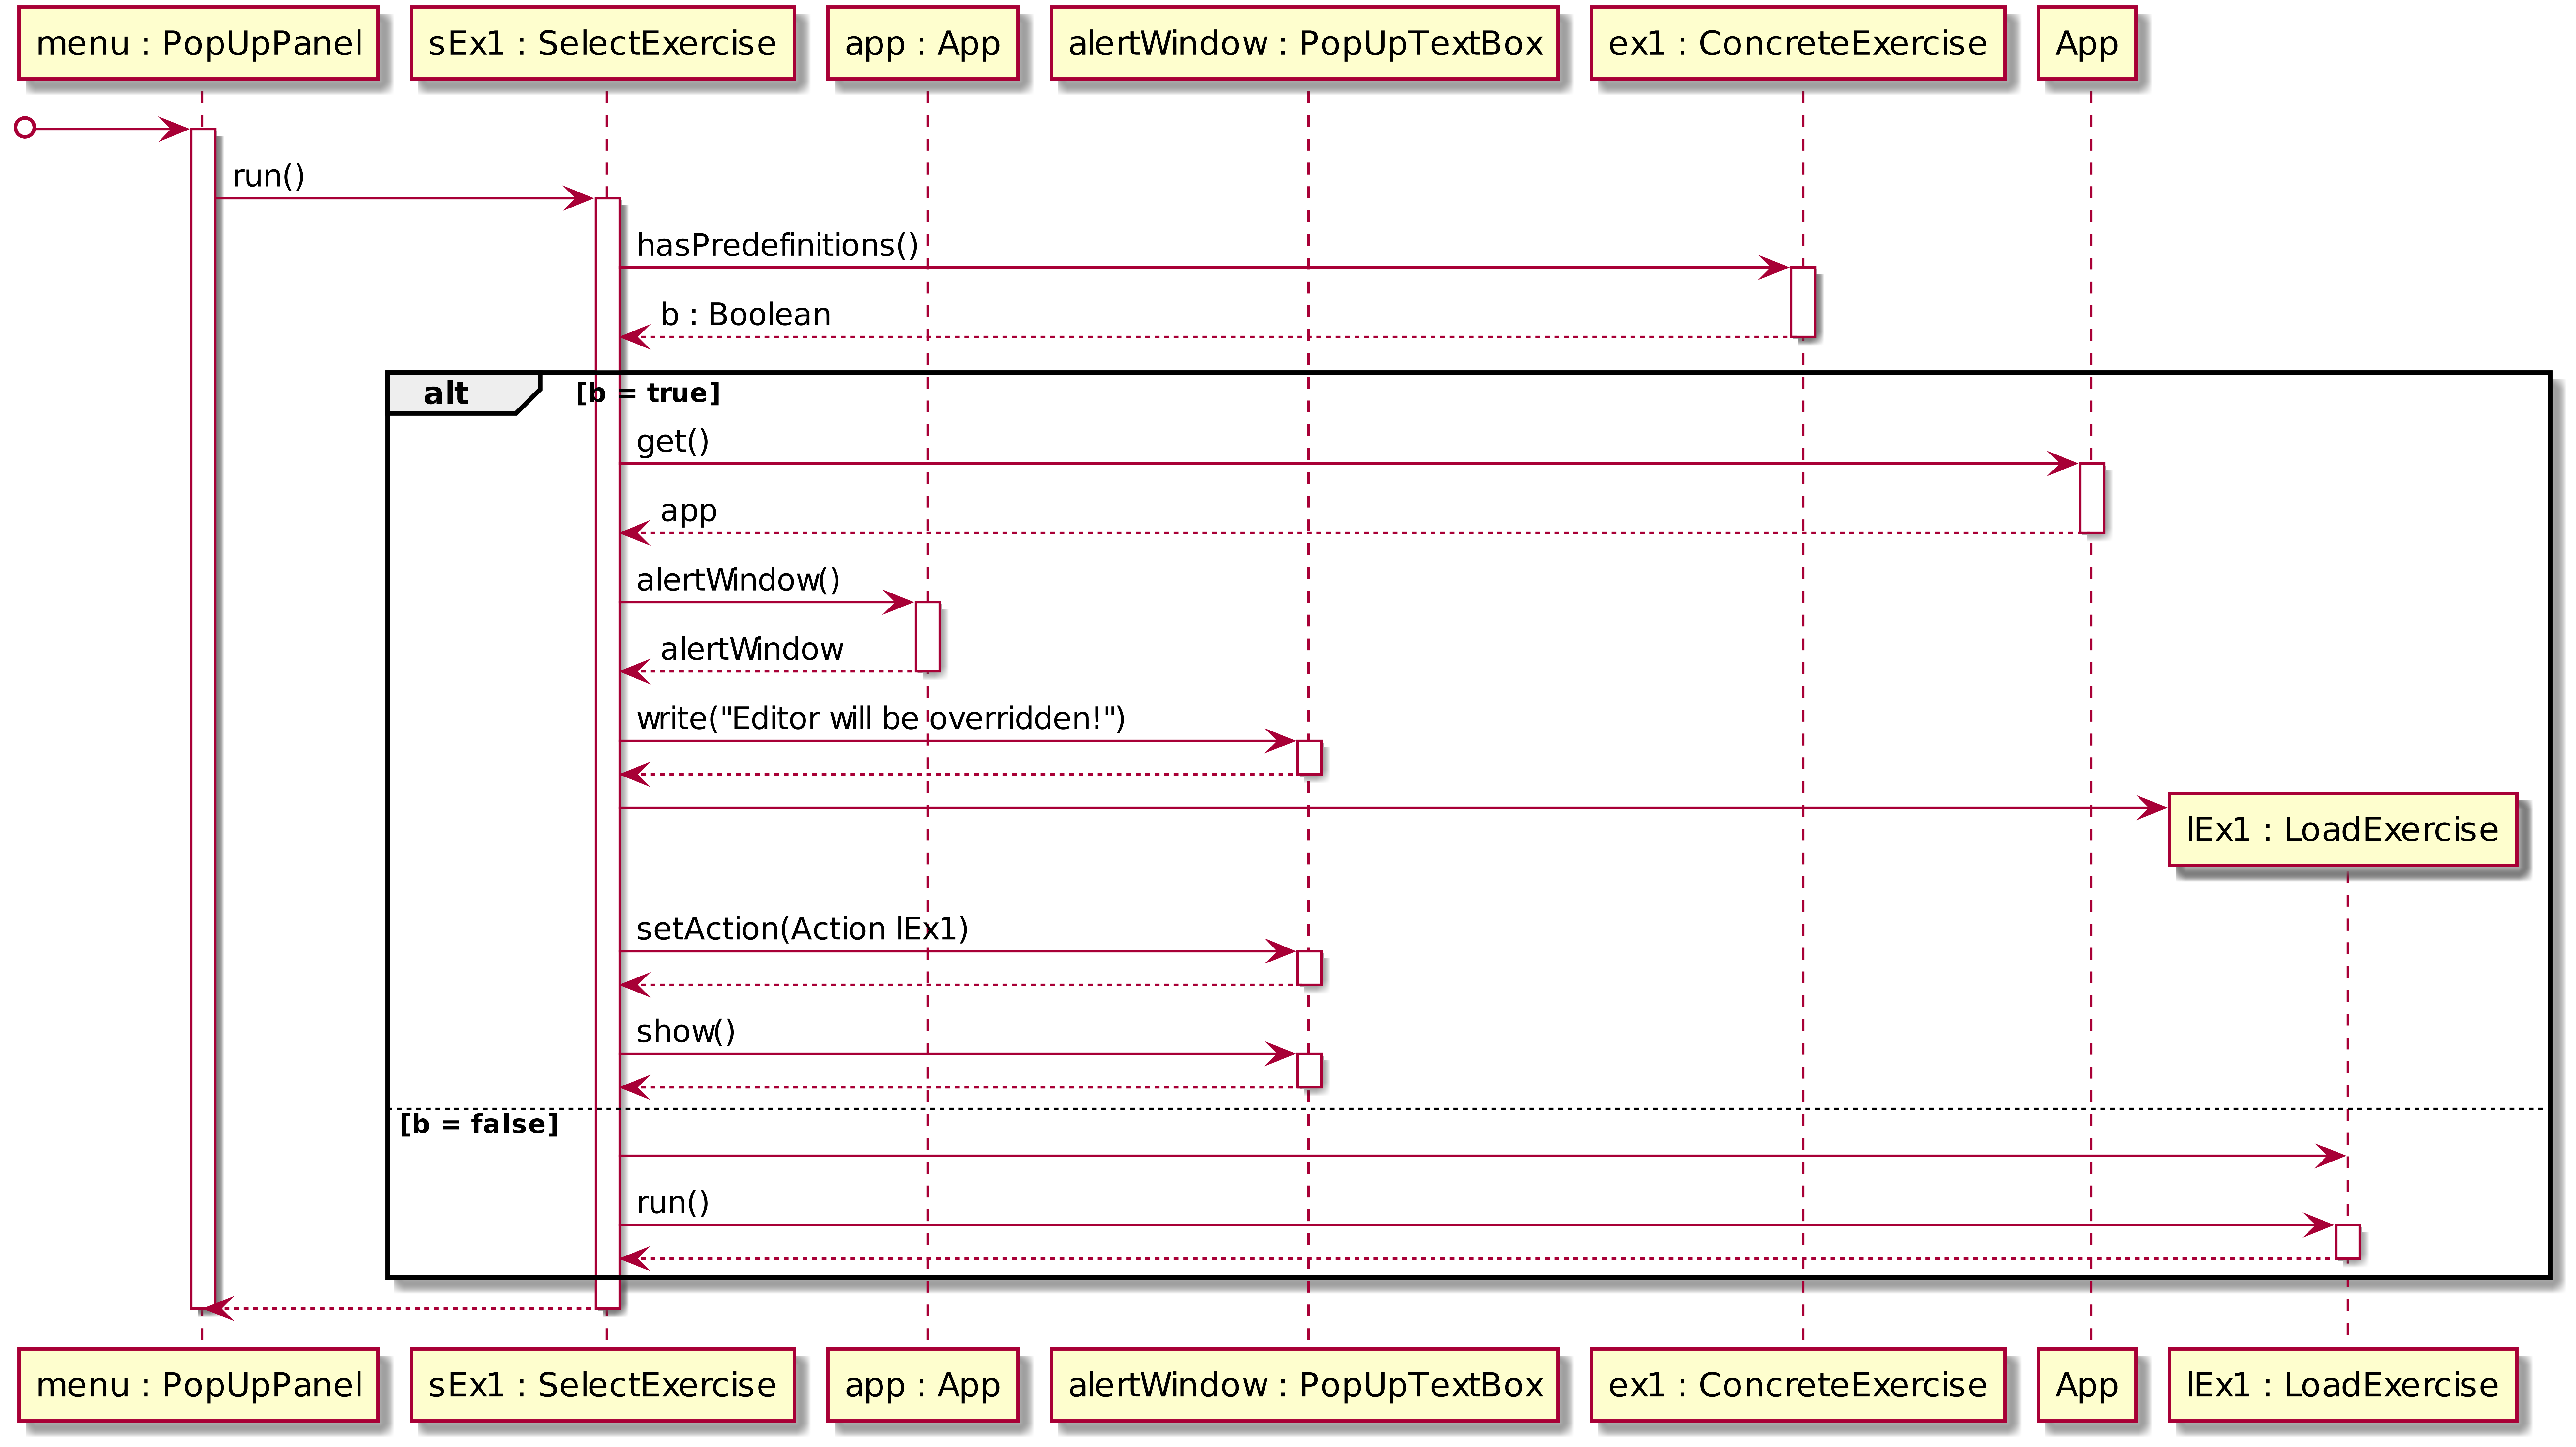
\includegraphics[width=\textwidth]{sequenceDiagrams/selectExercise}
	\caption{Sequenze diagram for selecting an exercise form the main menu.}
\end{figure}

\subsection{example action: load selected exercise}
The \texttt{\hyperref[type:edu.kit.wavelength.client.view.action.LoadExercise]{LoadExercise}} 
action loads a selected Exercise into the UI.

It updates the width of the Editor and displays \texttt{\hyperref[type:edu.kit.wavelength.client.view.webui.component.TextField]{TextField}}s 
that are responsible for displaying solution and explanation of the exercise.
The action also writes the correct content into the \texttt{\hyperref[type:edu.kit.wavelength.client.view.webui.component.TextField]{TextField}}s and updates the content of the \texttt{\hyperref[type:edu.kit.wavelength.client.view.webui.component.Editor]{Editor}} if necessary.

\begin{figure}[H]
	\centering
	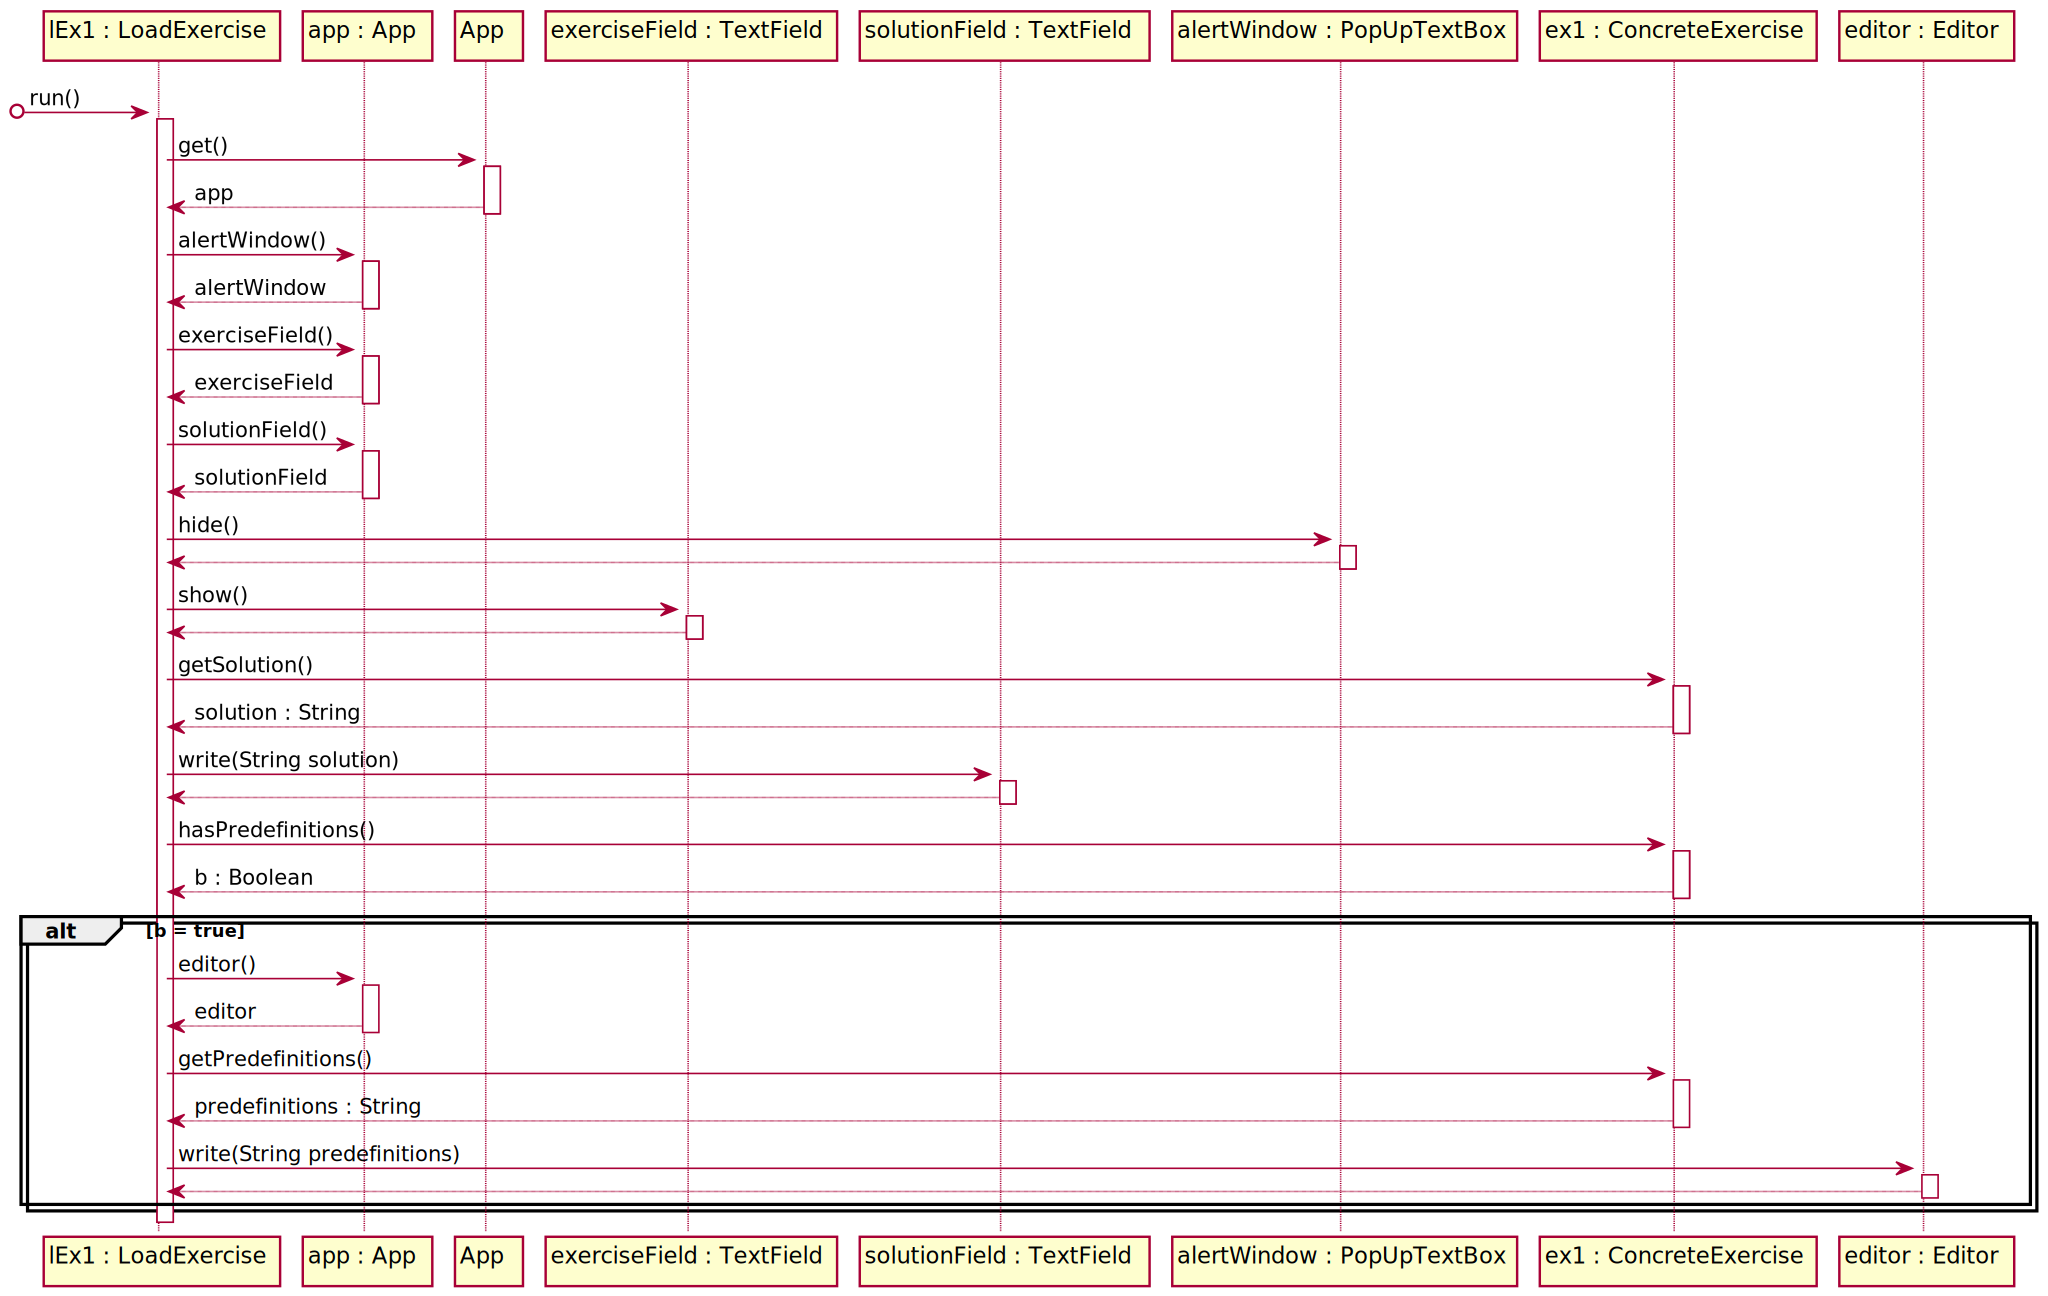
\includegraphics[width=\textwidth]{sequenceDiagrams/loadExercise}
	\caption{Sequenze diagram for loading a selected exercise into the UI}
\end{figure}

\subsection{Next term}
\label{sec:nt}
In order to retrieve the next redex to reduce from its reduction order, the
\texttt{\hyperref[type:edu.kit.wavelength.client.model.ExecutionEngine]{ExecutionEngine}}
calls the \texttt{next} method on the current reduction order. This method creates a new visitor which traverses
the lambda term, looking for the correct redex. In order to identify redexes,
specialized visitors that determine the type of a given lambda term are used.
These visitors extend \texttt{\hyperref[type:edu.kit.wavelength.client.model.term.NameAgnosticVisitor]{NameAgnosticVisitor}},
so that for example a named redex is still recognized as a redex.



\begin{figure}[H]
	\centering
	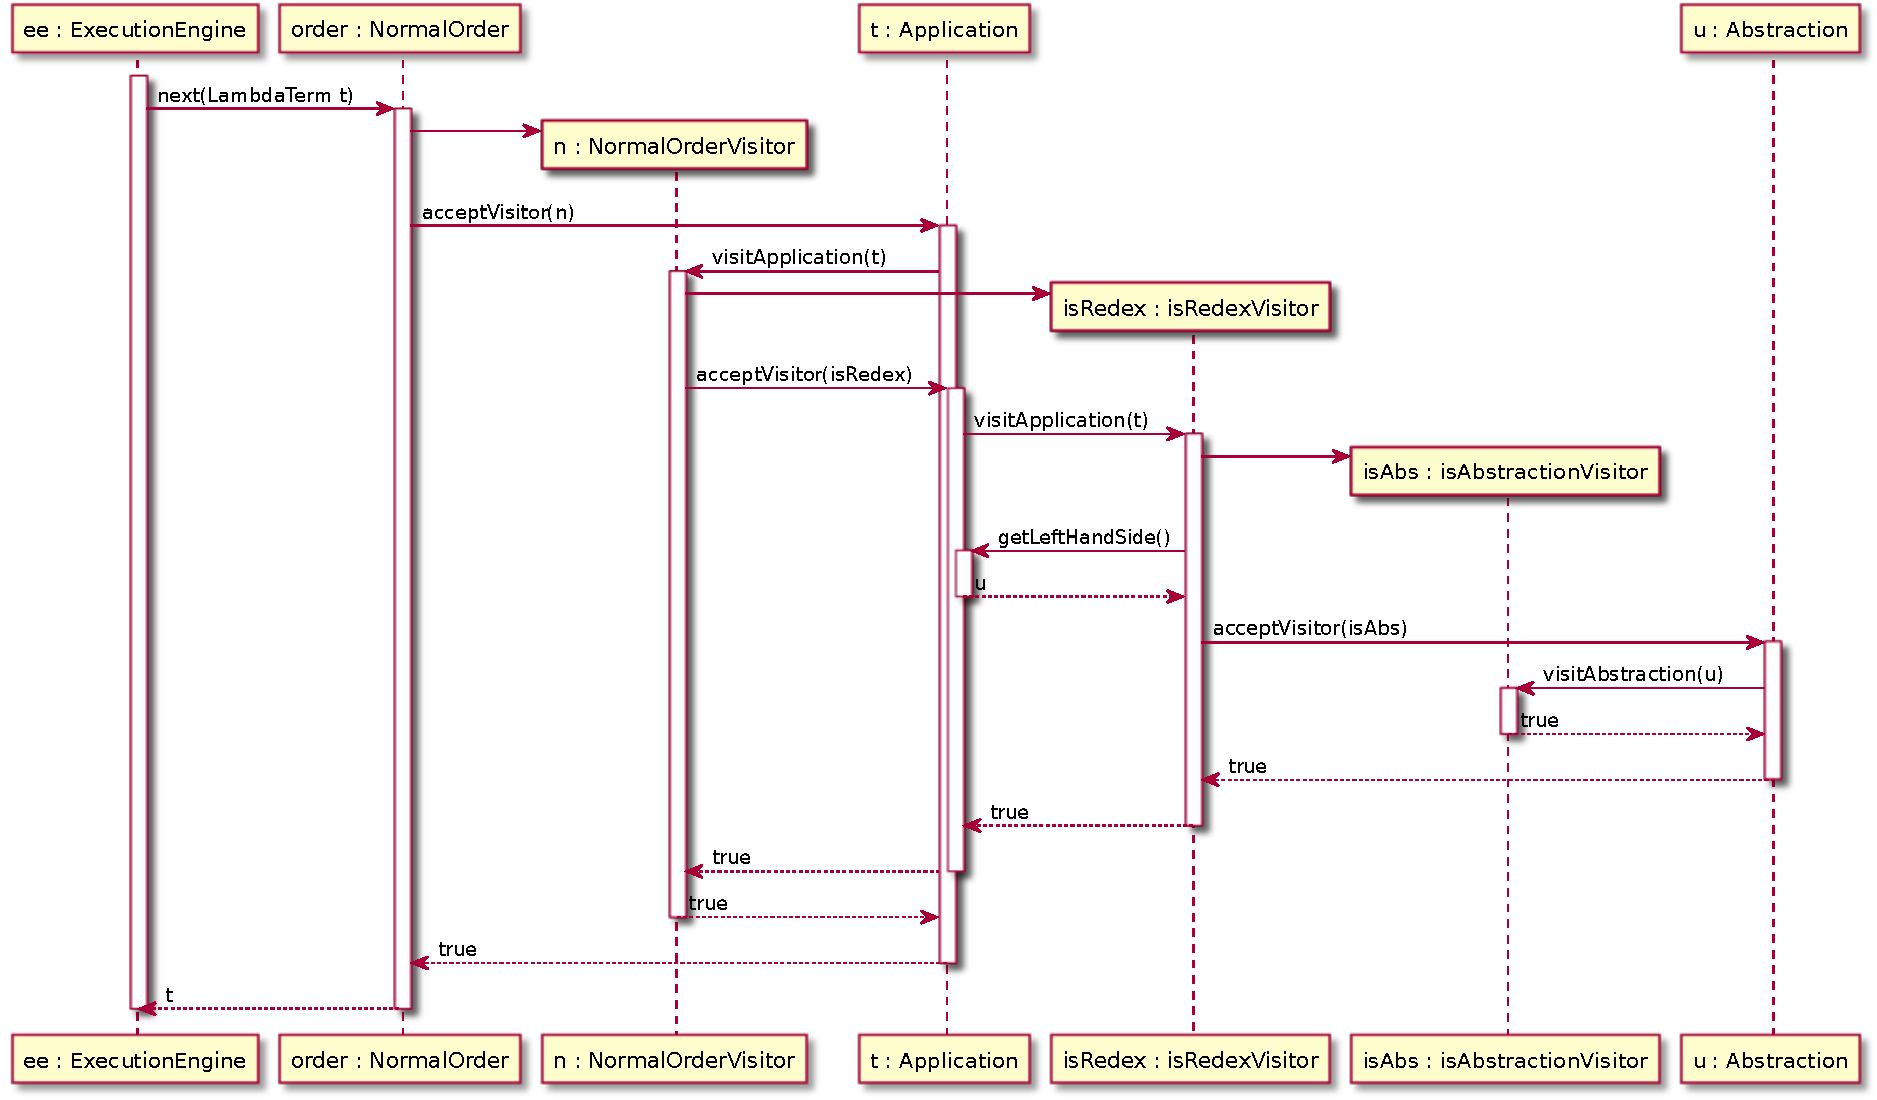
\includegraphics[width=\textwidth]{sequenceDiagrams/nextTerm}
	\caption{Sequence diagram for choosing the next term to reduce. In this example, we have $t = (\lambda x.x)(\lambda x.x)$ and $u = \lambda x.x$.}
\end{figure}


\subsection{$\beta$-reduction}
After the next redex to reduce has been retrieved from the reduction order (see \ref{sec:nt}),
the $\beta$-reduction of the redex can take place. Reduction is performed by the
\texttt{\hyperref[type:edu.kit.wavelength.client.model.term.BetaReducer]{BetaReducer}}
class, which traverses the tree and reassembles it unchanged until it finds the
redex returned by the reduction order. It then creates a
\texttt{\hyperref[type:edu.kit.wavelength.client.model.term.SubstitutionVisitor]{SubstitutionVisitor}}
which traverses the abstraction and performs the actual substitution. Both classes
extend \texttt{\hyperref[type:edu.kit.wavelength.client.model.term.TermTransformer]{TermTransformer}},
so they make sure that if they encounter a \texttt{\hyperref[type:edu.kit.wavelength.client.model.term.NamedTerm]{NamedTerm}}
whose body changed as a result of the substitution, the name tag is removed.


\begin{figure}[H]
	\centering
	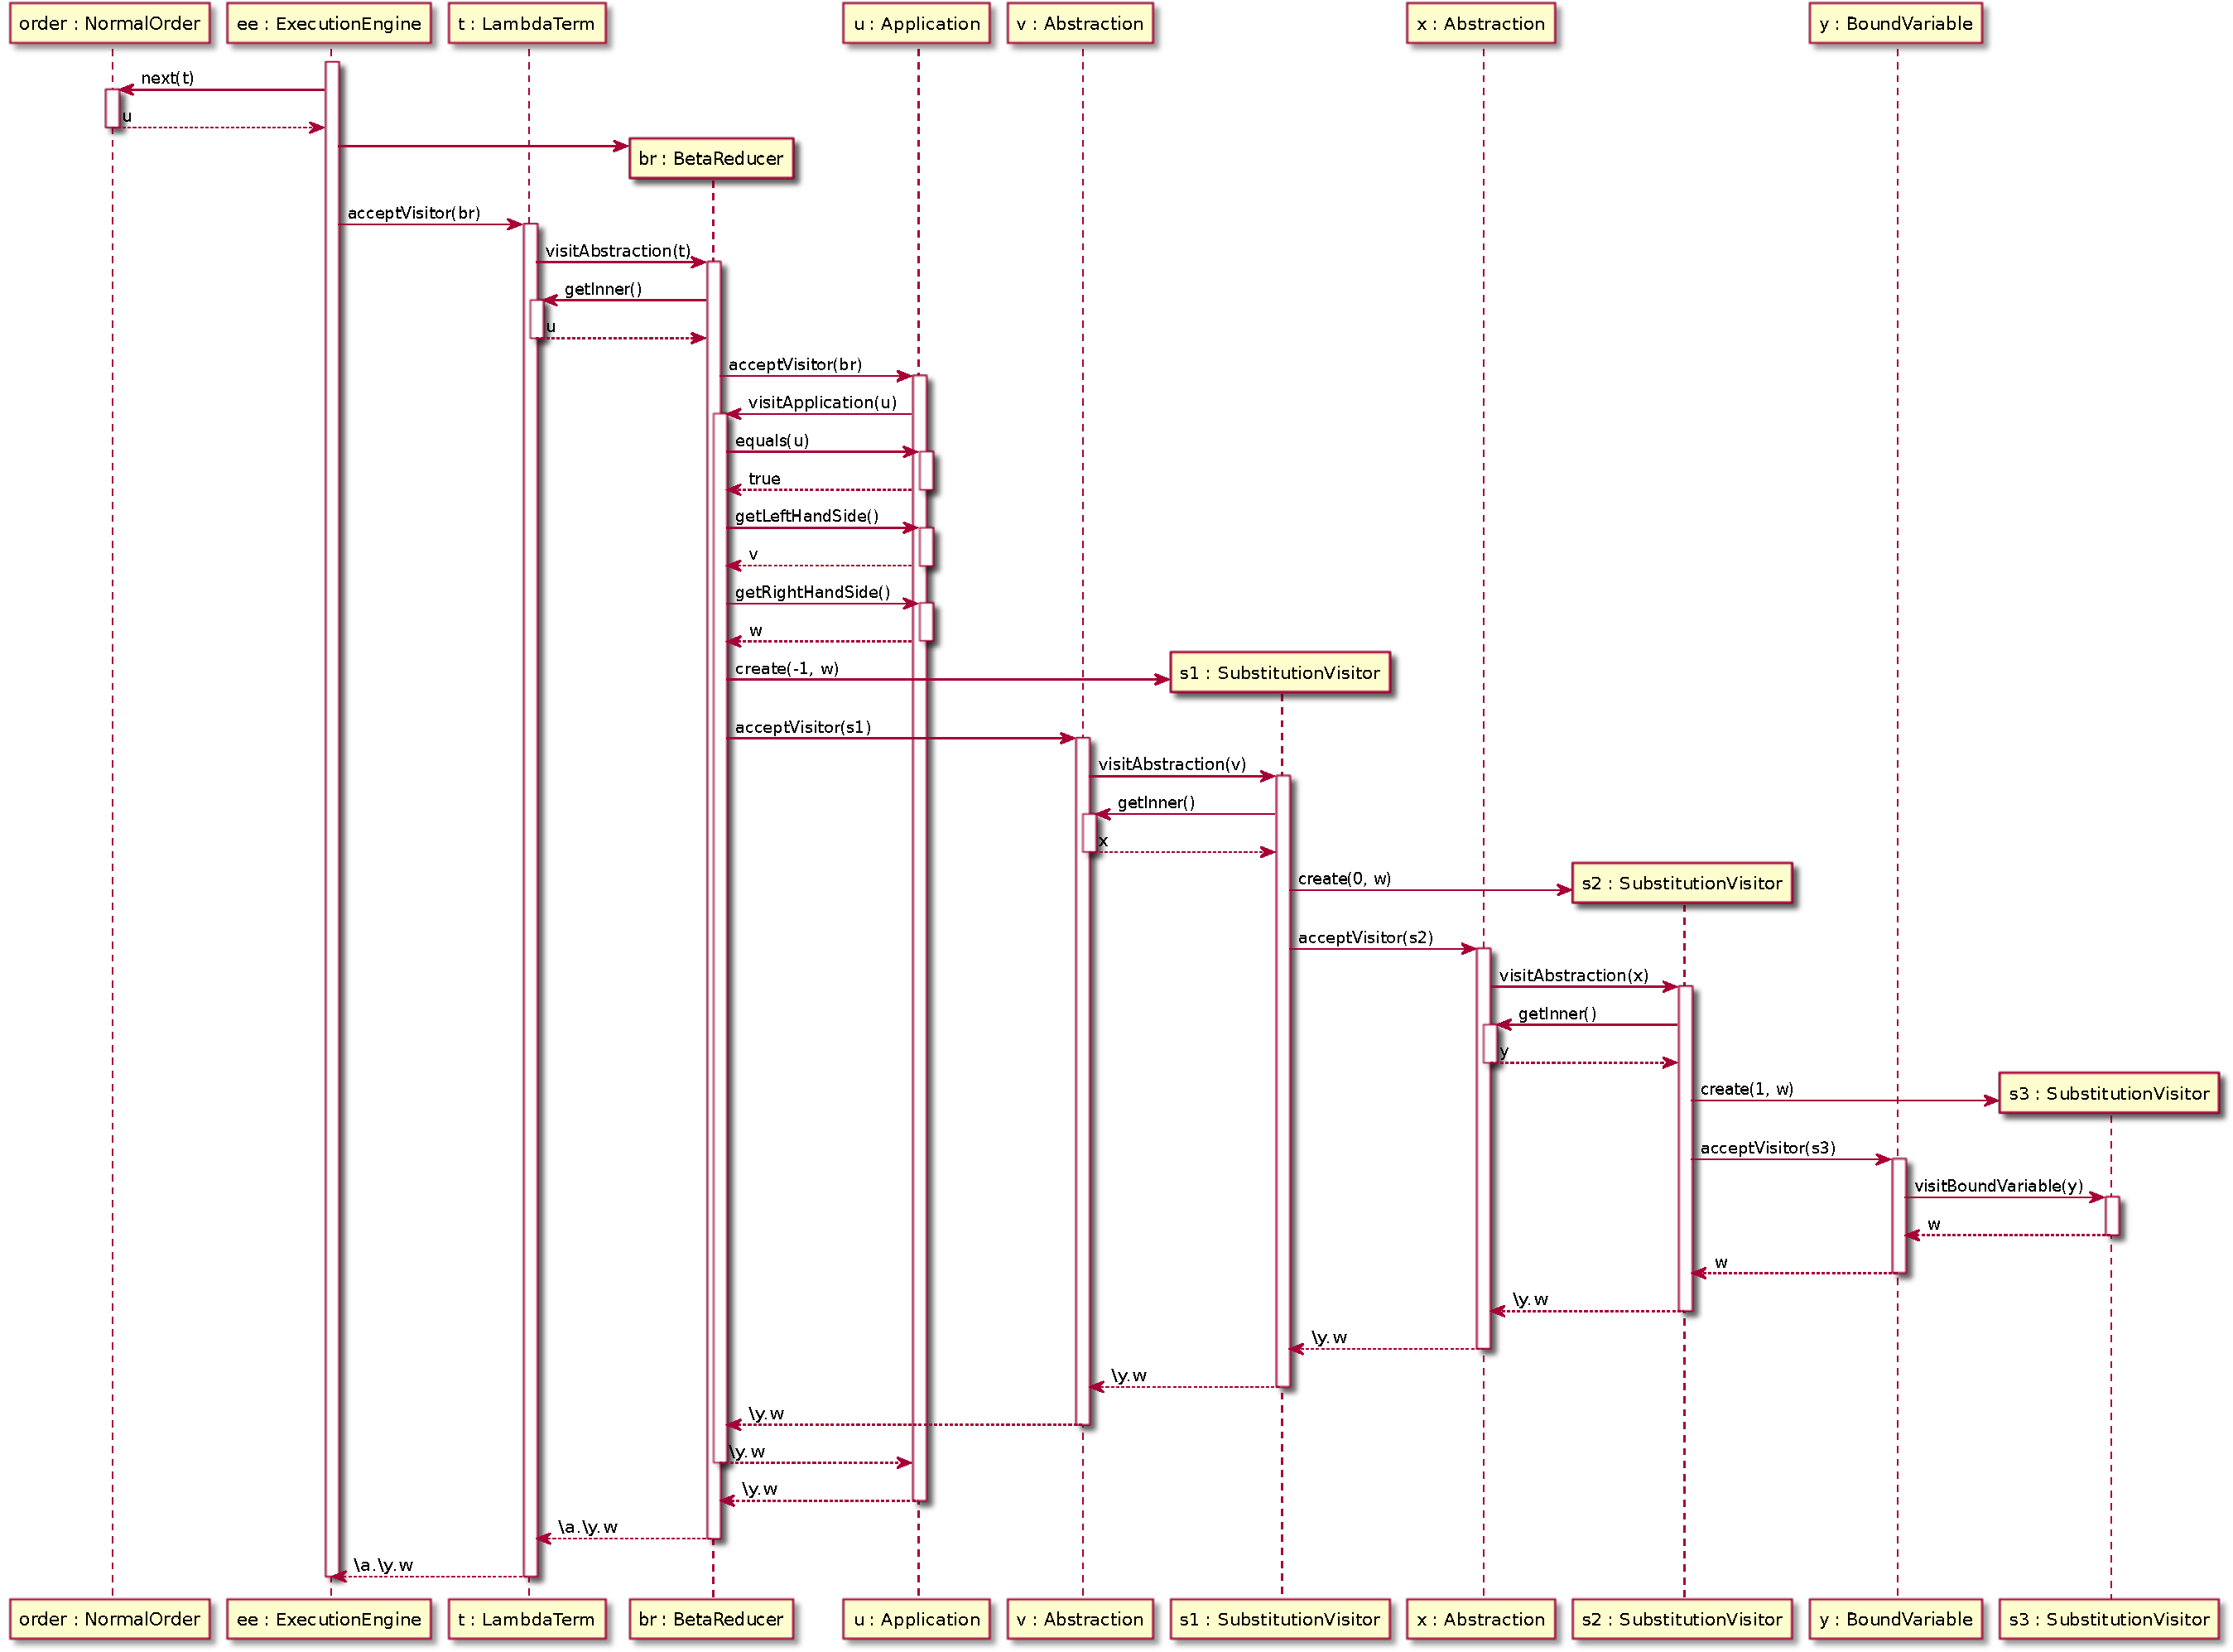
\includegraphics[width=\textwidth]{sequenceDiagrams/betaReduction}
	\caption{Sequence diagram for a $\beta$-reduction. In this example, we have $t = \lambda a.((\lambda x.\lambda y.x)(\lambda x.x))$,
		$u = (\lambda x.\lambda y.x)(\lambda x.x)$, $v = \lambda x.\lambda y.x$,
		$w = \lambda x.x$, $x = \lambda y.x$ and $y = x$. Note that in the terms called
		$x$ and $y$, the variable $x$ is actually represented as the De Bruijn index $2$
		(and not as a free variable).}
\end{figure}

